%BETTER TITLE
%TEAM NAME
%PROJECT NAME

%write a paragraph on the scripting langauage
%make gantt chart
\documentclass[a4paper,12pt]{article}

\addtolength{\oddsidemargin}{-.5in}
\addtolength{\evensidemargin}{-.5in}
\addtolength{\textwidth}{1in}
\addtolength{\topmargin}{-.875in}
\addtolength{\textheight}{1.75in}

\usepackage{graphicx}
\usepackage{multicol}
\usepackage{listings}
\lstset{language=Python} 

\begin{document}

\begin{titlepage}

  \newcommand{\HRule}{\rule{\linewidth}{0.5mm}}
  \begin{center}
    \textsc{\LARGE Project Proposal}\\[0.5cm] 
    \textsc{\large COSC 345 Assignment 1}\\[0.5cm] 
    %\textsc{\large COSC345 Assignment 1}\\[0.5cm]

    \HRule \\[0.6cm]
           { \huge \bfseries Five make a Shell}\\[0.4cm]
           \HRule \\[1.5cm]
           
           \Large \emph{Prepared by:}\\
           \begin{multicols}{3}
             Reuben \textsc{Crimp}\\
             Thomas \textsc{Hall}\\
             Richie \textsc{McKee}\\           
           \end{multicols}
           \begin{multicols}{2}
             Chris \textsc{McMillan}\\
             Shaun \textsc{Wratten}\\           
           \end{multicols}

  
  \null\vfill{\small April 4, 2014}\\[3cm]
    %\hline
    %\begin{center}
  \end{center}
\end{titlepage}
\section*{Project Overview}
%\end{center}
The shell will be a modern, POSIX style shell which will be released on linux, OSX and Windows under the FreeBSD License. The project will written almost entirely in C++ and all the source code will be released in it's entirety.

The Shell will be targeted at those of beginner level, people who are not particularly skilled at using a shell, and possibly even those who have never used one before.

The shell will be developed to be intuitive. Basic shell operations will be natural interactions, that most computer users are familiar with, anyone will be able to pick up our shell very quickly, even those from different OS backgrounds.

Despite the target audience of our Shell, it will still provide the full feature set that advanced users would expect.

Such features will include tab-completion, inline command prediction and detection, stream redirection, job control,  command history and aliases. Almost everything will be able to be customised.

It will also look pretty with proportional width font, no more ugly mono-spaced garbage, only beautifully kerned Helvetica.
\null\vfill

\section*{Introduction}
There are an excessive number of shells available for use in the world and the idea of coming along with something new, and better is extremely ambitious. When set with the task of designing and creating a new shell we spent a great deal of time looking at the most popular shells today to see what is was that made them popular, and if we could fathom any way in which we could make them better. We had a number of ideas that sprang to mind and a great deal more that became more apparent to us as we researched shells in greater detail and found things that we felt a shell would benefit from having.

We want a shell that has all the features of popular shells like the Bourne Again Shell. However we will attempt to add features that make it far more usable, especially for people less familiar with shells, but also people who like shortcuts. These features will include better mouse interaction support more intuitive directory navigation and file operations. 

In this proposal we shall present to you the main features of our shell including the tools and hardware that we will be required to work with such as IDEs, compilers and the physical machines that we will use.

%Xcode, C++ libraries and Cocoa graphic for OSX, vim, g++, C++ libraries and X11 for GNU/Linux, while with Windows we shall be working with Visual Studio 2013, C++ libraries and WIN32.

We have also anticipated a number of risks to our project such as the potential loss of a member, loss of code, or becoming overwhelmed by other demands or lack of experience. We will discuss how we hope to mitigate the chances of any of these occurring and how we shall cope if they do. 

Finally we have developed a project schedule, which has been laid out in a Gant chart, that will help to keep us on track, and help to alleviate some of the aforementioned risks. This schedule will hopefully give us something we can stick to but also be flexible. 

\pagebreak
\section*{The Team}

\subsection*{Reuben Crimp - \small Surgeon}
Reuben began programming in high school, making what interested him: games and websites. He graduated highschool in 2011 doing well in mathematics. He enrolled at Otago University in mid 2012, with computer science as a major, mathematics for a minor. He has very little industry experience but a strong passion for the subject matter.

\subsection*{Shaun Wratten - \small Co-pilot, C++ Expert}
Shaun recently graduated from UCOL in Palmerston North with a Bachelor’s degree in Information and Communications Technology,
%in which he learnt a decent portion of his skill set. This includes programming in
has has experience with
C\#, C++, scripting and web design using PHP and JavaScript, and working with MS-SQL and MySQL database. One of the major things he learned while studying was how to
%strutter ??
structure a team project and how to be as successful leader and team member.

\subsection*{Chris McMillan - \small Toolsmith, Objective-C Expert}
Chris has studied at the University of Otago since 2010, but only became interest in computers after high school. He completed a chemistry degree and then decided that his passion lay in computers and began study towards a computer science major as well. He will finish his BSc double major at the end of 2014. His main strengths are music and audiosoftware. Chris can confidently write in both Java and Python, but building a shell in C++ will be a challenge for him that he looks forward to and hopes to learn a lot from.

\subsection*{Thomas Hall - \small Tester, Language Architect}
Thomas is a recent graduate with BSc in Physics. He is currently studying a DipGrad in computer science to be finished in early 2015. He has experience programming in C\# from experimenting with Unity, and Matlab as part of his physics education. He also has a experience with Java and Python.

%Document guy
\subsection*{Richie McKee - \small Administrator, Editor and Program Clerk}
Richie completed his LLB/BA at the end of 2012 at Otago University. He always had a strong desire to learn computer science but is only now taking steps towards doing so. He began his DipGrad at the start of 2014 and hopes to be completed by the end of the year. As such his current level of experience is limited and his experience with programming is limited to what he learned during Summer School and what he is currently covering throughout the semester. To him the project is a daunting but exciting prospect that he hopes to learn from.

\pagebreak
\section*{Tools and Hardware}

Our development enviroment will be the lab machines with OSX and GNU/linux.
Our windows dev enviroment will be our own private windows 7 64-bit machine.
\subsection*{Development tools}
\begin{multicols}{3}
  \subsubsection*{Windows}
  Visual Studio 2013 \\
  C++ libraries \\
  WIN32 \columnbreak
  \subsubsection*{OSX}
  Xcode \\
  C++ libraries \\
  Cocoa graphics \columnbreak
  \subsubsection*{GNU/Linux}
  vim, g++ \\
  C++ libraries \\
  X11
\end{multicols}
\subsection*{Revision Control}
We will use git for our distributed revision control, with project hosting by github.com.
\section*{The Shell}
This shell will be released on linux, OSX and windows, and will come with several usability enhancements which are described in follwing sections, as well as most of the features you'd expect from a modern shell.
\begin{multicols}{4}
  \noindent
  Stream redirection \\
  Piping \\
  Tab completion \\
  Command history \\
  Job control \\
  Aliases \\
  Directory stack
\end{multicols}
\subsection*{Modularised Code}

The diagram below shows the modules we plan to implement, but more importantly how input gets handled and processed.

\begin{center}
  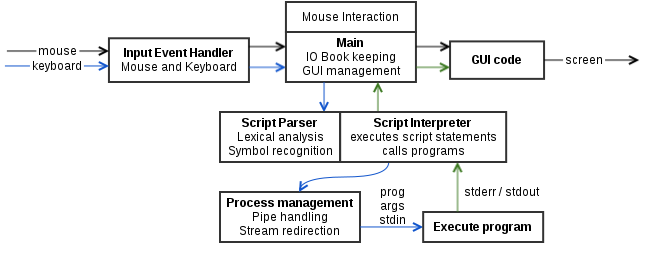
\includegraphics[width=16cm]{shellflow.png}\\
  \small Fig 0 - Flow of information through our shell
\end{center}

\pagebreak
%\subsection{Cross OS file support}
%Different operating systems by convention define a new line within a file differently
%We will allow the user to choose how to handle cross platform files

%\begin{tabular}{l | l}
%Fix & edit as current OS, save as current OS (Forced when parsing a script) \\
%Compatibility & edit as current OS, save as original. \\
%Do nothing & edit as original save as original. \\
%Custom & Fix; but you can specify the replacement terminator \\
%{‘\textbackslash r’, ‘\textbackslash n’, ‘\textbackslash r \textbackslash n’, ‘\textbackslash n \textbackslash r’}
%\end{tabular}

\subsection*{Usability Features}
The shell will allow for intuitive mouse interactions, these interactions will be very similar to the actions in a standard GUI OS environment (i.e. double click for open).

However, most of our actions won't actually perform the action outright, instead it will paste the command that would perform the requested action into the current prompt, i.e. clicking "delete file" in a *nix environment will paste the command "rm \textless file-name\textgreater" into the prompt, the user will then have to press "return" to execute the command.

The purpose of this is to help the user if they do not know the specific text command, and then to teach that particular command to them.

\begin{center}
  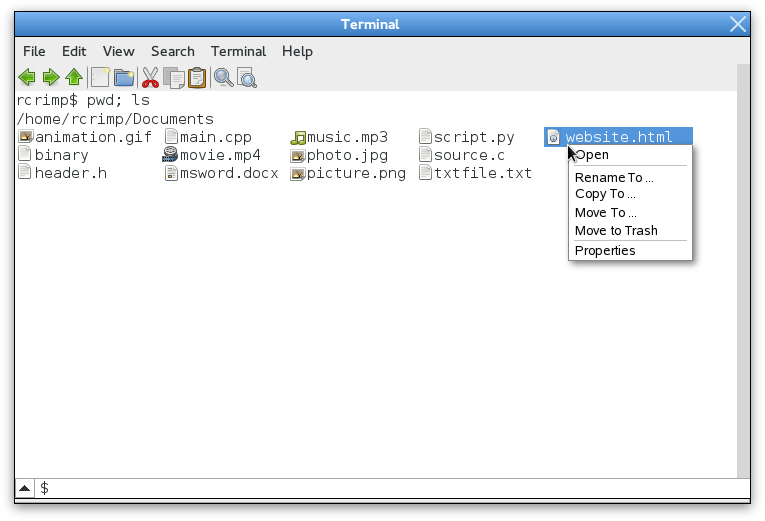
\includegraphics[width=13cm]{context.png}\\
  \small Fig 1 - Graphical ls with context menu
\end{center}
\subsection*{Intuitive directory navigation}
Our shell will come with an inbuilt 'ls' function, designed specifically to aid beginners
(which is replaceable with the OS default ls/dir)\\*
File-names will be preceded by a filetype icon, like a GUI shell, see (fig.1)\\

Clicking on a directory will paste the command "cd \textless dir-name\textgreater" into the prompt.\\*
Double clicking a directory will execute the command "cd \textless dir-name\textgreater".\\*
Right clicking on a directory will open a context menu (see fig.1), which will list basic directory commands e.g "open (cd)", "move to .. (mv), clicking on these will paste the corresponding command into the prompt.
\subsection*{Intuitive file interaction}
Single, double and right clicking on a file, will exhibit similar results to clicking on a directory.
Single clicking on a file will paste the ``\textless file-name\textgreater'' into the current prompt.
Double clicking on a file will open the file with the OS default application (if one exists).

Right clicking a file will also  open a context menu with similar commands listed (move, rename, delete, open etc....)

\begin{center}
  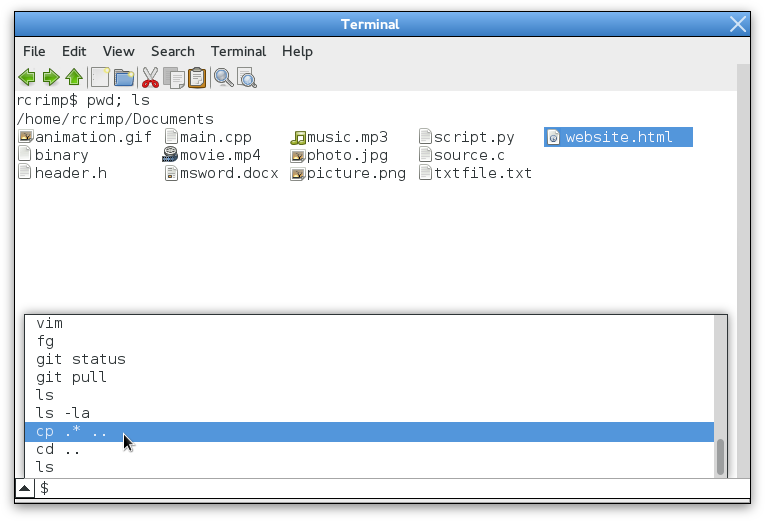
\includegraphics[width=13cm]{history.png}\\
  \small Fig 2 - Interactive history
\end{center}

\subsection*{The Toolbar}
Just below the menu bar there will be a toolbar for useful shell commands.

Hovering over each button wil present the user with it's name and the command used to execute the command.

e.g hovering over ``new folder'' will show ``New Folder : \$ mkdir \textless dir-name\textgreater''. \\

\noindent
Fig 2 has the following buttons from left to right.

\begin{multicols}{4}\noindent
  Previous Dir \\ %``dir-stack alias'' \\
  Next Dir \\ %``dir-stack alias'' \\
  Up one Dir \\*%``cd ..'' \\
  \columnbreak

  \noindent
  New File \\ %``touch \textless file-name\textgreater'' \\
  New Folder \\*%``mkdir \textless dir-name\textgreater'' \\
  \columnbreak

  \noindent
  Cut Text \\ %``Ctrl-'' \\
  Copy Text \\ %``Ctrl-'' \\
  Paste Text \\*%``Ctrl-'' \\
  \columnbreak

  \noindent
  Search for a file \\ %``word'' \\
  Search in a file \\*%``word'' \\
\end{multicols}

\subsection*{Interactive command history}
Clicking the small arrow to the left of the prompt, will open a drop down menu (upwards), showing the last commands executed in ascending order, allowing for easy access

The standard bash style keyboard shortcuts to access your history will also exist for the
more advanced user. (up, down, "!!", ``!str" etc...)

\subsection*{Directory Bookmarks}
We will allow users to set directory bookmarks with a quick command.

Executing ``set \#work'' will set a bookmark in the current directory called "work", then executing ``\#work'' will change the users directory back to directory in which it was set.\\*
So quick navigation between commonly accessed directories when working on a project.\\[0.5cm]
We will also implement a directory stack, for the more technically savvy user.\\*
``\#back'' and ``\#forward'' will be reserved for intuitive interaction with  directory stack, which will match the ``back'' and ``forward'' buttons on the toolbar.


\pagebreak
\subsection*{Tab Completion}

Pressing the tab key will attempt to complete the current unfinished symbol written in the prompt, i.e tabbing on ``rmdir Docu'' will try and complete the ``Docu'' symbol.\\
For example: ``Documents'', if such a directory exists.

The completions for a symbol will be dependent on the current content of the symbol and what the shell is expecting, e.g. if the shell expects the current symbol to be a file, then the shell will only search for files.

\subsubsection*{Tab-tab}
If there are multiple possible completions for the current symbol we write all of these completions to the console, letting the user view their choices.

After writing all completions for the current symbol, successive tabbing  won't redundantly list them out again (like BASH), instead we will cycle through the possible completions inline in the prompt.  

\subsubsection*{Wild card}
Our shell will treat a '*' in the prompt as a ``wild card'', i.e * will lazily match any string, even the empty string. \\
so ``*.c'' would match ``source.c'', ``main.c'' and even ``.c''

\subsubsection*{Parent directories}

The parent directories of the working directory will be included when completing a directory name, so navigating back up a file structure is easier.

No longer will you need to ``cd ../../../../''

\subsection*{If we have time}
More rigorous pattern recognition, using wildcards can be very powerful, but more fine grained filtering would be nice - maybe.\\[0.5cm]
A tab complete function for man pages, i.e ``man 3 *fpr'' would complete the last symbol as ``printf'',  ``fprintf'' ...\\[0.5cm]
Active command prediction, which attempt to complete the current command from the users command history, show in figure 3. 

\begin{center}
  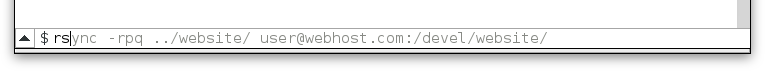
\includegraphics[width=14cm]{autocomplete.png}\\
  \small Fig 3 - predictive complete
\end{center}

\pagebreak
\section*{Script Syntax}
Since no one in our group has ever made an interpreter before, we have gone for a very simple language.

We will take advantage of whitespace, to make things easier to tokenize, but we will not use whitespace indentation to indicate code blocks.

The end of a statement (line) will be indicated by either a newline character or a semi-colon.

\begin{multicols}{2}

  \subsubsection*{Keywords}
  \begin{tabular}{| l | l | l | l | } \hline
    and & fail & if & return \\ \hline
    break & false & in & true \\ \hline
    class & for & not & try \\ \hline
    else & function & or & while \\ \hline
    end & global &  print &  \\ \hline
  \end{tabular}

  \subsubsection*{Arithmetic operators}
  \begin{tabular}{| l | l | } \hline
    + & Addition \\ \hline
    - & Subtraction \\ \hline
    * & Multiplication \\ \hline
    \textbackslash & Division \\ \hline
    \% & Modulus \\ \hline
    \(\wedge\)  & Exponent \\ \hline
  \end{tabular}

  \subsubsection*{Assignment operators}
  \begin{tabular}{| l | l | } \hline
    = & Simple assignment  \\ \hline
    += & Add and assignment  \\ \hline
    -= & Subtract and assignment  \\ \hline
  \end{tabular}

  \subsubsection*{Comparison Operators}
  \begin{tabular}{| l | l | } \hline
    == & Equal \\ \hline
    != & Not equal \\ \hline
    \textgreater & Left larger \\ \hline
    \textless & Right Larger \\ \hline
    \textgreater= & Left larger than or equal to \\ \hline
    \textless= & Right larger than or equal to \\ \hline
  \end{tabular}

\end{multicols}

\subsection*{Code Examples}
\begin{multicols}{2}
  \subsubsection*{Loops}
  \begin{lstlisting}
    for ( j = 0;  j < 5; j ++ ) :
       echo i
    end
    
    i = 0
    while ( i < 5 ) :
       echo i
       i++
    end

  \end{lstlisting}
  \columnbreak
  \subsubsection*{if function}
  \begin{lstlisting}
    function foo ( x ) :
       if ( x == 0 ) :
          bar()
          baz()
       else:
          qux( x )
          foo( x - 1 )
       end
    end
  \end{lstlisting}
\end{multicols}

\pagebreak
\section*{Risk Analysis}

We wanted to implement a proactive approach to dealing with risks as opposed to a reactive approach.

Our objective is to be able to avoid risk whenever possible, and to solve problems before they manifested themselves. This preparation would hopefully mean that we could respond to problems that did occur in a controlled and effective manner. We understand that risks evolve throughout the course of the project and so we will be constantly monitoring identified risks throughout the course of the year via a risk map to ensure that we are still keeping them at bay. 

\subsection*{Loss of a Team Member}
The consequences of losing a team member are fairly straightforward. We would lose 20\% of our workforce if this occurs. However the effect of losing a person would be vastly different depending on who was lost. For example, losing Reuben or Shaun would would be worse because they are responsisble for most of the programming. But if such drastic events occured we would survive, Tom is also an adept programming so is Chris.

As it stands there are no foreseen reasons as to why our team would lose a member. Everyone plans on completing the course. However it is possible Richie might leaves for a more secure job. But his role  could be split between Thomas and Chris in the event of his departure. 

\subsection*{Concurrent Working}
We will have multiple people modiying the same files which could cause conflicts. Thankfully this risk is all but eliminated since we are using Git which detects file conflicts.

\subsection*{Failure to Complete Milestones}
Due to the the requirements that the shell work across a number of platforms, our group is required to have a fairly extensive knowledge on a number of technologies. The time spent learning how to use these tools is time we are not coding and testing.

We have assigned certain tasks to certain team members, and it is there responsibility to ensure their task is completed.\\

\begin{tabular}{l l}
  Reuben & Linux GUI,  process stream redirection/piping \\
  Shaun & Windows GUI, command prediction/completion \\
  Chris & GUI Architect, Mac OSX GUI \\
  Thomas & Script Lexical Analyser/Parser \\
  Richie & Planning, Documenting and testing \\
\end{tabular}\\*

If anything is behind schedule, then it is up to the person responsible to request help on IRC, or mention it on one of our bi-weekly meeetings.\\

Workload from other classes may get in the way, it is a real possibility that team members may be so busy that they are unable to carry out their duties. Which is why our regular meeting and IRC are so important.
\pagebreak
\section*{Project Schedule}
Monitoring the project and ourselves is an important way for us to anticipate future problems and gives us a chance to avoid them.

The key to completing this project is to stay on schedule, and if problems arise, we communicate so we can get back on schedule.

\subsection*{Full Project}
Here's the full plan in a Gantt chart, from now until release
\begin{center}
  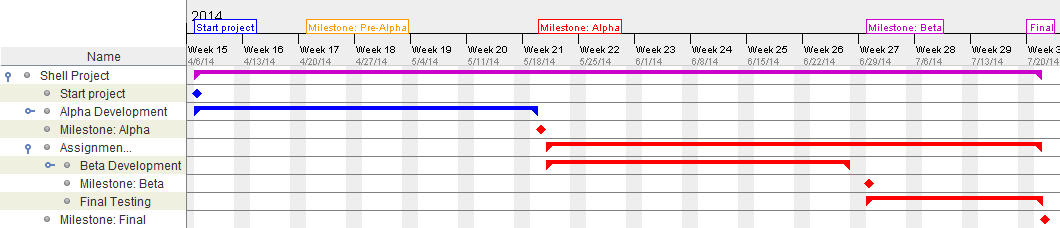
\includegraphics[width=16cm]{full.png}\\
\end{center}

\subsection*{Alpha}
And here's the first segment expanded, from now until when the alpha release.
\begin{center}
  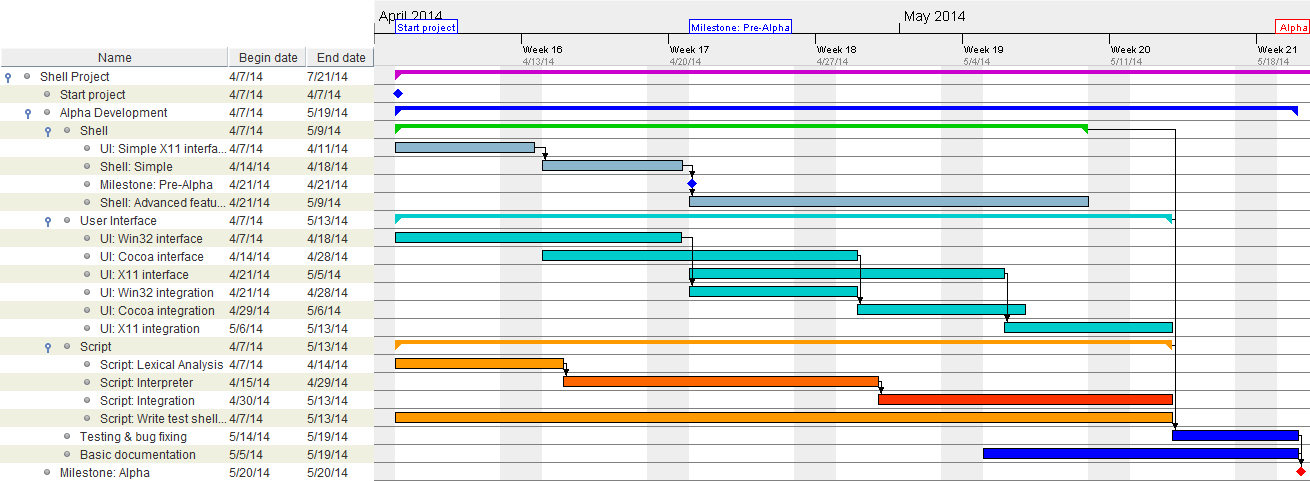
\includegraphics[width=16cm]{alpha.png}\\
\end{center}

\end{document}
